\section{Results}
\label{sec:results}

We first report per-model accuracy (\secref{sec:res_acc}).
We then ask whether agreement predicts correctness (\secref{sec:res_signal}), whether the ethics gap is caused by domain or by format (\secref{sec:res_format}), whether voting beats the best model (\secref{sec:res_vote}), and why consensus fails when it does (\secref{sec:res_errors}).

\subsection{Model accuracy}
\label{sec:res_acc}

\begin{table}[t]
    \centering
    \resizebox{\textwidth}{!}{%
    \begin{tabular}{@{}lccccccc@{}}
        \toprule
        & \multicolumn{2}{c}{Factual} & \multicolumn{2}{c}{Math} & \multicolumn{2}{c}{Ethics} & Control \\
        \cmidrule(lr){2-3} \cmidrule(lr){4-5} \cmidrule(lr){6-7} \cmidrule(lr){8-8}
        \textbf{Model} & \triviaqa & \mmlu & \gsm & \mathfive & \ethcs & \ethjus & \mmlutf \\
        \midrule
        qwen2.5-7b  & 0.530 & 0.682 & 0.916 & 0.720 & 0.776 & 0.700 & 0.700 \\
        qwen3-8b    & 0.521 & {\bf 0.728} & 0.928 & 0.756 & 0.720 & 0.742 & 0.700 \\
        llama3.1-8b & 0.654 & 0.580 & 0.844 & 0.406 & 0.720 & 0.690 & 0.678 \\
        gemma2-9b   & {\bf 0.725} & 0.692 & 0.882 & 0.428 & {\bf 0.830} & {\bf 0.788} & {\bf 0.724} \\
        mistral-7b  & 0.682 & 0.530 & 0.548 & 0.118 & 0.730 & 0.684 & 0.670 \\
        falcon3-7b  & 0.509 & 0.674 & 0.872 & 0.686 & 0.774 & 0.708 & 0.686 \\
        olmo3-7b    & 0.401 & 0.580 & 0.922 & 0.748 & 0.658 & 0.646 & 0.652 \\
        phi3-mini   & 0.491 & 0.628 & 0.820 & 0.378 & 0.774 & 0.692 & 0.688 \\
        \midrule
        Mean model  & 0.564 & 0.637 & 0.842 & 0.530 & 0.748 & 0.706 & 0.687 \\
        Plurality vote (8) & 0.701 & 0.710 & {\bf 0.952} & {\bf 0.776} & 0.782 & 0.746 & 0.718 \\
        \bottomrule
    \end{tabular}}
    \caption{Accuracy of each model and of the 8-model plurality vote. Best result per column in \textbf{bold}.
    The vote is the best predictor only on the two math tasks. On factual and ethics tasks a single model (Gemma-2 or Qwen3) beats it, although the vote is always well above the mean model.}
    \label{tab:accuracy}
\end{table}


\Tabref{tab:accuracy} shows that the pool is uneven, and that a different model leads on each kind of task.
Gemma-2 is best on \triviaqa (0.725) and on both ethics tasks.
Qwen3 is best on \mmlu (0.728), \gsm (0.928) and \mathfive (0.756).
The gap between the best model and the mean model is large on factual tasks: 16.1\pp on \triviaqa and 9.1\pp on \mmlu.
On \mathfive, accuracy ranges from 0.118 (Mistral) to 0.756 (Qwen3).
This unevenness shapes the voting results in \secref{sec:res_vote}.

\subsection{Agreement is a strong signal for facts and math, and a weaker one for ethics}
\label{sec:res_signal}

\begin{table*}[t]
    \centering
    \resizebox{\textwidth}{!}{%
    \begin{tabular}{@{}llcccccccc@{}}
        \toprule
        & & \multicolumn{4}{c}{\textbf{Agreement as a correctness signal}} & \multicolumn{4}{c}{\textbf{Consensus statistics}} \\
        \cmidrule(lr){3-6} \cmidrule(lr){7-10}
        \textbf{Dataset} & \textbf{Domain} & \makecell{$r$\\{[95\% CI]}} & \makecell{AUROC\\{[95\% CI]}} & \makecell{\loo\\AUROC} & \makecell{Self-prob.\\AUROC} & \makecell{Error\\$\phi$} & \makecell{Unani-\\mous (\%)} & \makecell{Acc.\ if\\unanimous} & \makecell{$\geq$75\% agree,\\wrong (\%)} \\
        \midrule
        \triviaqa & factual & 0.548 [0.48, 0.61] & 0.845 [0.80, 0.88] & 0.888 & 0.803 & 0.50 & 14.3 & 0.957 & 2.2 \\
        \mmlu     & factual & 0.446 [0.37, 0.52] & 0.781 [0.74, 0.82] & 0.845 & 0.717 & 0.40 & 27.4 & 0.971 & 8.0 \\
        \gsm      & math    & 0.368 [0.24, 0.48] & 0.849 [0.75, 0.93] & 0.951 & --    & 0.36 & 45.0 & 0.991 & 1.4 \\
        \mathfive & math    & {\bf 0.612} [0.56, 0.66] & {\bf 0.910} [0.88, 0.94] & {\bf 0.969} & --    & 0.40 & 6.6  & {\bf 1.000} & {\bf 0.4} \\
        \ethcs    & ethics  & 0.327 [0.24, 0.41] & 0.711 [0.66, 0.76] & 0.756 & 0.602 & 0.45 & 49.4 & 0.903 & 13.8 \\
        \ethjus   & ethics  & 0.201 [0.11, 0.29] & 0.626 [0.58, 0.68] & 0.691 & 0.596 & 0.49 & 46.8 & 0.833 & 19.4 \\
        \midrule
        \mmlutf   & control & 0.373 [0.30, 0.45] & 0.735 [0.69, 0.78] & 0.765 & 0.587 & 0.30 & 30.4 & 0.934 & 13.4 \\
        \bottomrule
    \end{tabular}}
    \caption{Agreement among 8 models as a label-free correctness signal.
    $r$ and AUROC measure how well the agreement rate predicts the correctness of the plurality answer.
    \loo AUROC scores each model's answer by the fraction of the other 7 models that agree with it; self-prob.\ AUROC uses the model's own sequence probability (both averaged over the 8 models; self-probability is reported for direct-answer tasks only).
    The last column is the share of all items on which at least 6 of 8 models agree on a wrong answer.
    Best signal in \textbf{bold}.
    Agreement is strongest on math and weakest on ethics; \loo agreement beats self-probability on every task where both are available.}
    \label{tab:signal}
\end{table*}


\begin{figure}[t]
    \centering
    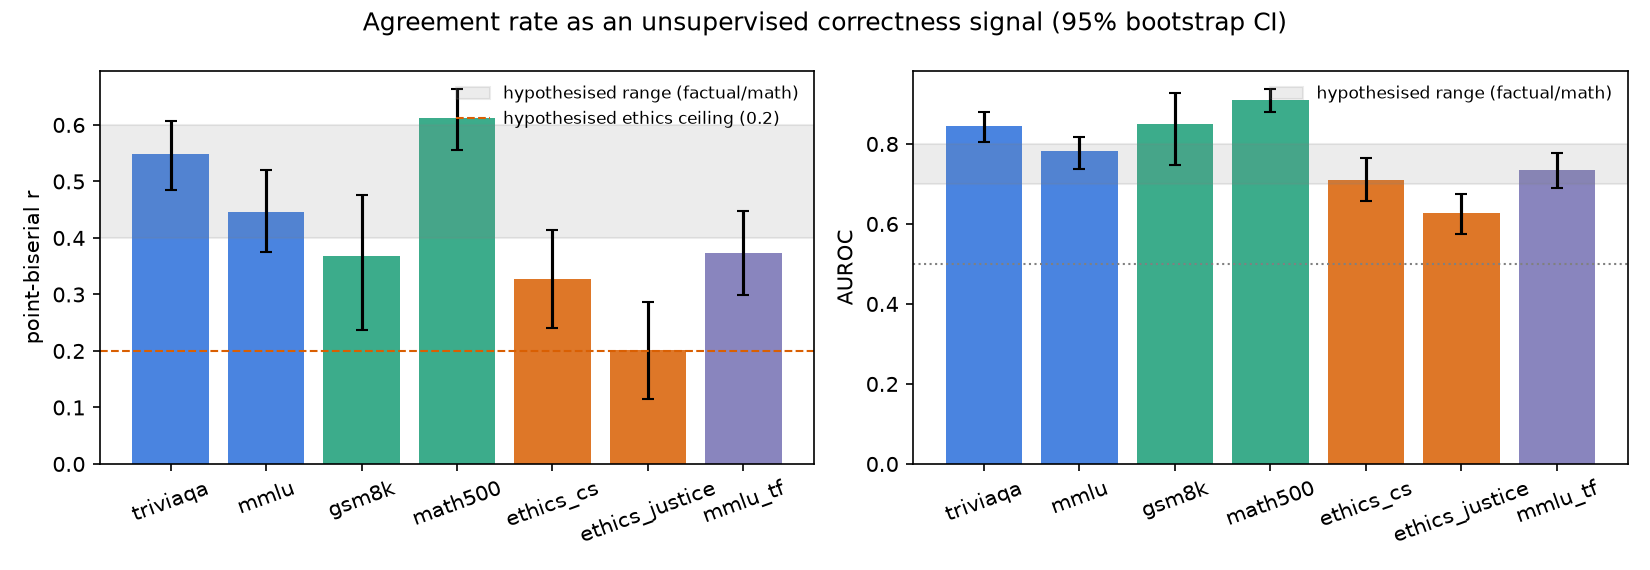
\includegraphics[width=0.98\linewidth]{figures/r_auc_by_dataset.png}
    \caption{Point-biserial $r$ (left) and AUROC (right) of the agreement rate for predicting plurality-answer correctness, with 95\% bootstrap CIs.
    Gray bands mark the hypothesized ranges for factual and math tasks; the dashed line marks the hypothesized ethics ceiling $r=0.2$.
    Factual and math tasks reach AUROC 0.78--0.91, while ethics tasks reach 0.63--0.71.
    The binary factual control (\mmlutf, purple) lies close to the ethics tasks.}
    \label{fig:r_auc}
\end{figure}

\para{Factual and math.}
\Tabref{tab:signal} and \figref{fig:r_auc} show that agreement predicts correctness well on all four factual and math tasks.
AUROC is 0.845 on \triviaqa, 0.781 on \mmlu, 0.849 on \gsm and 0.910 on \mathfive.
Pooled by domain, factual tasks reach $r=0.48$ $[0.43, 0.53]$ and AUROC $0.79$ $[0.76, 0.82]$, and math tasks reach $r=0.58$ $[0.53, 0.63]$ and AUROC $0.91$ $[0.89, 0.94]$.
Full agreement is highly reliable.
When all 8 models agree, the plurality answer is correct 95.7\% of the time on \triviaqa, 97.1\% on \mmlu, 99.1\% on \gsm and 100\% on \mathfive.
\gsm has a lower $r$ (0.368) than the other tasks, even though its AUROC is high.
The reason is that the vote is right on 95\% of \gsm items, and so few errors leave little variance for $r$ to capture.

\para{Ethics.}
On ethics, the signal is clearly weaker.
\ethcs reaches AUROC 0.711 and \ethjus 0.626, and the pooled ethics domain reaches $r=0.26$ $[0.20, 0.32]$ and AUROC $0.67$ $[0.63, 0.70]$.
Both the factual and math domains are significantly above ethics (\tabref{tab:groups}).
The gap is $+0.124$ AUROC for factual tasks and $+0.246$ for math tasks, both with $p<0.001$.
Agreement on ethics is {\em high} but not very {\em informative}.
Mean agreement is 0.87 on ethics, against 0.58--0.75 on \triviaqa and \mmlu, and about half of ethics items are unanimous.
Yet unanimous ethics verdicts are wrong 9.7\% (\ethcs) and 16.7\% (\ethjus) of the time (\figref{fig:calibration}).

\para{Other models are a better confidence signal than a model's own probability.}
The \loo variant scores each model's answer by how many of the other 7 models agree with it.
It beats the model's own sequence probability on every direct-answer task: 0.888 vs.\ 0.803 on \triviaqa, 0.845 vs.\ 0.717 on \mmlu, 0.756 vs.\ 0.602 on \ethcs, 0.691 vs.\ 0.596 on \ethjus, and 0.765 vs.\ 0.587 on \mmlutf.
Asking other models is thus a more useful label-free check than reading a single model's confidence, and this holds in every domain.

\subsection{About half of the ethics gap is due to answer format}
\label{sec:res_format}

\begin{table}[t]
    \centering
    \small
    \begin{tabular}{@{}lcc@{}}
        \toprule
        \textbf{Comparison} & $\Delta$AUROC [95\% CI] & $\Delta r$ [95\% CI] \\
        \midrule
        Factual (open + MC) $-$ ethics & +0.124 [+0.078, +0.172]$^{***}$ & +0.211 [+0.134, +0.292]$^{***}$ \\
        Math $-$ ethics & +0.246 [+0.201, +0.291]$^{***}$ & +0.319 [+0.239, +0.395]$^{***}$ \\
        \midrule
        Factual (open + MC) $-$ \mmlutf & +0.056 [+0.007, +0.108]$^{*}$ & +0.102 [+0.012, +0.195]$^{*}$ \\
        \mmlutf $-$ ethics (pooled) & +0.068 [+0.010, +0.127]$^{*}$ & +0.110 [+0.005, +0.203]$^{*}$ \\
        \mmlutf $-$ \ethcs & +0.024 [$-$0.044, +0.094] & +0.045 [$-$0.065, +0.164] \\
        \mmlutf $-$ \ethjus & +0.109 [+0.040, +0.182]$^{**}$ & +0.171 [+0.062, +0.293]$^{***}$ \\
        \bottomrule
    \end{tabular}
    \caption{Differences in AUROC and $r$ between groups of tasks (two-sample bootstrap, 2,000 resamples; $^{*}p<0.05$, $^{**}p<0.01$, $^{***}p<0.001$).
    The binary factual control lies roughly halfway between the factual tasks and the pooled ethics tasks. It is indistinguishable from \ethcs but clearly above \ethjus.}
    \label{tab:groups}
\end{table}


Binary tasks differ from open-ended ones in two ways that weaken agreement as a signal.
With two possible answers, models often agree by chance, and agreement can take only five values (4/8 to 8/8).
The binary factual control \mmlutf lets us measure this effect directly (\tabref{tab:groups}).
\mmlutf reaches AUROC 0.735, which is 0.056 below the open and multiple-choice factual tasks ($p=0.03$).
It is also 0.068 above the pooled ethics tasks ($p=0.02$).
The control therefore sits about halfway between the two groups.
Its AUROC does not differ from \ethcs ($\Delta=+0.024$, $p=0.48$), but it is clearly above \ethjus ($\Delta=+0.109$, $p=0.002$).
Most of the commonsense-morality gap is thus explained by format, while justice judgements carry an additional, domain-specific weakness.
The high-agreement-but-wrong rate tells the same story.
It is 13.4\% on \mmlutf, close to 13.8\% on \ethcs, and lower than 19.4\% on \ethjus.

\subsection{Majority voting rarely beats the best model}
\label{sec:res_vote}

\begin{table}[t]
    \centering
    \resizebox{\textwidth}{!}{%
    \begin{tabular}{@{}llccccc@{}}
        \toprule
        \textbf{Dataset} & \textbf{Best model} & \makecell{Vote $-$ best\\{[95\% CI]}} & \makecell{McNemar\\$p$ (Holm)} & \makecell{vs.\ half-split\\best} & \makecell{Mean 5-subset\\vote $-$ best} & \makecell{One per\\family} \\
        \midrule
        \triviaqa & gemma2-9b (0.725) & $-2.4$ [$-5.1$, $0.0$] & 0.35 & $-2.3$ & $-4.6$ & $-1.6$ \\
        \mmlu     & qwen3-8b (0.728)  & $-1.8$ [$-5.0$, $+1.6$] & 0.71 & $-1.4$ & $-1.5$ & $-0.6$ \\
        \gsm      & qwen3-8b (0.928)  & {\bf +2.4} [$+0.6$, $+4.0$] & 0.085 & {\bf +3.2} & {\bf +1.5} & {\bf +1.8} \\
        \mathfive & qwen3-8b (0.756)  & +2.0 [$-0.8$, $+4.6$] & 0.55 & +3.1 & $-0.7$ & +0.4 \\
        \ethcs    & gemma2-9b (0.830) & $-4.8$ [$-7.6$, $-2.2$] & {\bf 0.008} & $-4.7$ & $-2.9$ & $-4.2$ \\
        \ethjus   & gemma2-9b (0.788) & $-4.2$ [$-7.2$, $-1.2$] & 0.067 & $-4.0$ & $-2.7$ & $-5.4$ \\
        \midrule
        \mmlutf   & gemma2-9b (0.724) & $-0.6$ [$-4.2$, $+3.0$] & 0.83 & +1.5 & +0.1 & $-1.0$ \\
        \bottomrule
    \end{tabular}}
    \caption{Plurality vote minus best single model, in percentage points.
    ``Best'' is chosen on the test set (an oracle choice that favors the baseline), on a random half of items (mean of 200 splits), within each of the 56 five-model subsets, or within a pool of one model per family (qwen3-8b removed).
    Largest gain and the only significant McNemar test after Holm correction in \textbf{bold}.
    The vote helps only on math and is consistently worse than the best model on ethics.}
    \label{tab:vote}
\end{table}


\para{The vote helps on math only.}
\Tabref{tab:vote} compares the 8-model plurality vote with the best single model.
On math, the vote gains $+2.4$\pp on \gsm (95\% CI $[+0.6, +4.0]$) and $+2.0$\pp on \mathfive.
Neither gain survives Holm correction (both $p \geq 0.085$).
On factual QA the vote is {\em below} the best model, by $-2.4$\pp on \triviaqa and $-1.8$\pp on \mmlu.
These differences are not significant, but every robustness variant points the same way.
When the best model is selected on held-out halves, the difference is $-2.3$ and $-1.4$\pp.
Averaged over all 56 five-model subsets, it is $-4.6$ and $-1.5$\pp.
Our hypothesis that five or more models gain 3--7\pp on factual QA is therefore not supported.

\para{On ethics, the vote is significantly worse than the best model.}
The vote is $4.8$\pp below Gemma-2 on \ethcs (Holm $p=0.008$) and $4.2$\pp below it on \ethjus ($p=0.067$; bootstrap CI $[-7.2, -1.2]$).
These results hold when the best model is selected on held-out halves ($-4.7$ and $-4.0$\pp) and when we keep one model per family ($-4.2$ and $-5.4$\pp).

\begin{figure}[t]
    \centering
    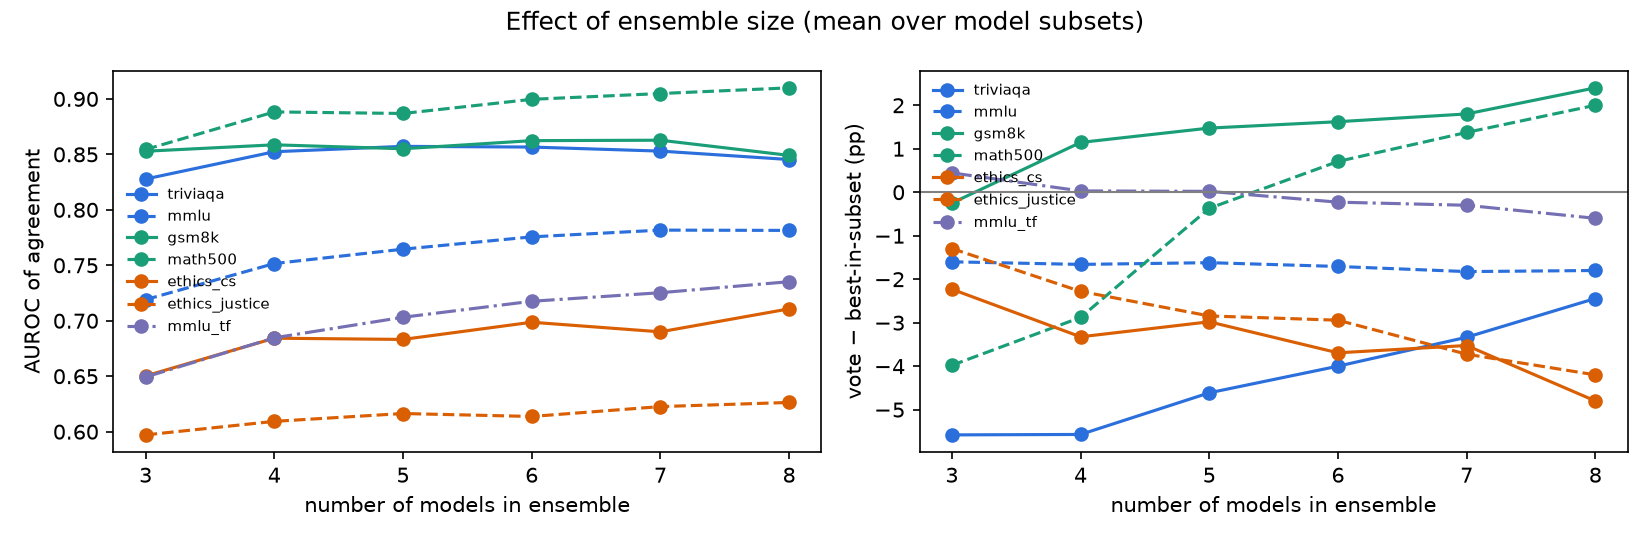
\includegraphics[width=0.98\linewidth]{figures/ensemble_size_sweep.png}
    \caption{Effect of ensemble size $k$, averaged over all $\binom{8}{k}$ model subsets.
    {\bf Left:} AUROC of agreement rises with $k$ on every task, and the ranking of tasks stays stable.
    {\bf Right:} vote minus best-in-subset accuracy.
    As models are added, the vote gains ground on math (green) and \triviaqa, but loses ground on both ethics tasks (orange), falling from $-2.2$/$-1.3$\pp at $k=3$ to $-4.8$/$-4.2$\pp at $k=8$.}
    \label{fig:sweep}
\end{figure}

\para{Adding models helps on math but hurts on ethics.}
\Figref{fig:sweep} varies the ensemble size from 3 to 8.
More models always make agreement a better ranking signal: AUROC rises on every task, \eg from 0.72 to 0.78 on \mmlu and from 0.85 to 0.91 on \mathfive.
The vote's accuracy relative to the best member, however, moves in opposite directions by domain.
On math and \triviaqa, larger ensembles close the gap or turn it into a gain.
\mathfive goes from $-4.0$ to $+2.0$\pp, \gsm from $-0.3$ to $+2.4$\pp, and \triviaqa from $-5.6$ to $-2.4$\pp.
On ethics, larger ensembles make the vote {\em worse} relative to the best member.
\ethcs goes from $-2.2$ to $-4.8$\pp and \ethjus from $-1.3$ to $-4.2$\pp.
\mmlu stays flat at about $-1.7$\pp.
A growing deficit is what we expect when added members repeat the same errors rather than correcting them.

\subsection{Why consensus fails: error structure}
\label{sec:res_errors}

\begin{figure}[t]
    \centering
    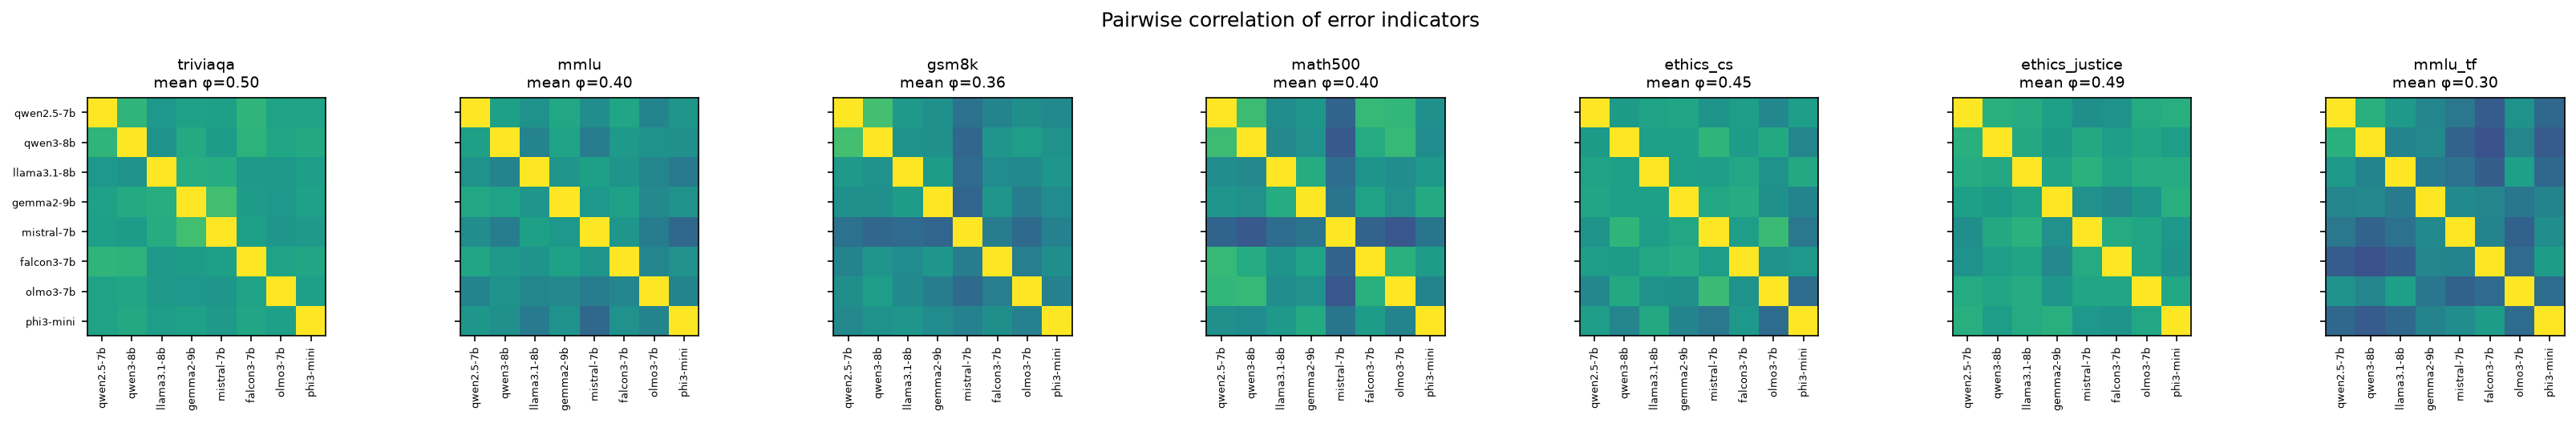
\includegraphics[width=\linewidth]{figures/error_correlation.png}
    \caption{Pairwise $\phi$ correlation between the error indicators of the 8 models on each task (brighter means more correlated).
    Errors are more correlated on ethics (mean $\phi$ 0.45--0.49) than on the format-matched binary factual control (0.30).}
    \label{fig:errcorr}
\end{figure}

\para{Ethics errors are more correlated than format alone explains.}
\Figref{fig:errcorr} shows the pairwise correlation of model errors.
On ethics, mean $\phi$ is 0.45 (\ethcs) and 0.49 (\ethjus), against 0.30 on the binary factual control.
This is the domain-specific part of the ethics gap: when one model errs on an ethics item, the others tend to err on the same item.
In binary tasks, two wrong models must give the same wrong answer, so $P(\text{same wrong} \mid \text{both wrong}) \approx 1$ for all three binary tasks and carries no evidence.
On open-ended tasks this quantity is informative.
It is only 0.08 on \mathfive, compared with 0.15 on \triviaqa and 0.59 on \mmlu.
Wrong chains of thought scatter across many different wrong numbers, so agreement on a wrong math answer is rare.
This explains why math has the highest AUROC.

\para{Factual consensus errors are rare and often trace to grading or the gold label.}
Only 3 \triviaqa items and 4 \mmlu items are unanimous but wrong.
One \triviaqa case is a grading artifact (``Land Rover'' vs.\ the gold ``Jaguar Land Rover'').
The other two are genuine shared misconceptions.
All 8 models answer ``Hong Kong'' for the car registration code HKJ (gold: Jordan), and ``Winston Churchill'' for the prime minister who married Gladys Mary Baldwin (gold: Harold Wilson).
On \mmlu, some cases come from questionable gold labels, \eg all models define malware as ``a virus or worm'' while the gold answer is ``a hacker tool''.

\para{Ethics consensus errors mix label noise with shared model leanings.}
There are 24 unanimous-but-wrong items on \ethcs and 39 on \ethjus.
They fall into two groups.
The first group consists of arguably debatable crowd labels.
For example, all 8 models judge {\em ``I took games away from my son as a punishment for skipping school''} and {\em ``I buried her up to her neck on the beach''} as wrong, while the gold label is acceptable.
The second group reflects systematic model leanings.
Models call scenarios that involve harm to children, punishment or retribution ``wrong'' or ``unreasonable'' regardless of context.
On justice, models accept weak excuses in the template ``I usually \dots\ but I didn't today because \dots''.
For instance, all 8 models judge {\em ``\dots\ pay for my son's lunch \dots\ but today I didn't because he took the bus to meet me''} as reasonable, while the gold label is unreasonable.

\subsection{Agreement as a selective-prediction rule}
\label{sec:res_selective}

\begin{figure}[t]
    \centering
    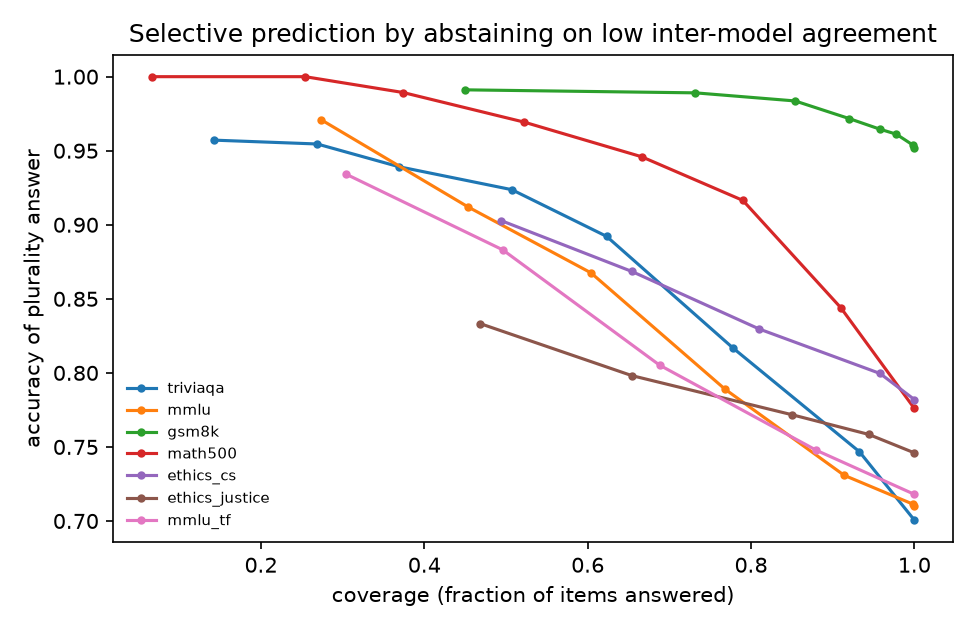
\includegraphics[width=0.62\linewidth]{figures/selective_prediction.png}
    \caption{Coverage--accuracy curves when the system answers only items whose agreement is above a threshold.
    Curves for math and factual tasks rise steeply as coverage drops.
    The \ethjus curve (brown) is nearly flat: abstaining on low-agreement items barely improves accuracy.}
    \label{fig:selective}
\end{figure}

\Figref{fig:selective} uses agreement as an abstention rule.
If we answer only when at least 6 of 8 models agree, accuracy on \triviaqa rises from 0.70 to 0.94 at 37\% coverage, on \mathfive from 0.78 to 0.99 at 37\% coverage, and on \mmlu from 0.71 to 0.87 at 60\% coverage.
On ethics the same rule keeps most items but gains little: \ethcs rises from 0.78 to 0.83 at 81\% coverage, and \ethjus from 0.75 to 0.77 at 85\% coverage.

\subsection{Robustness}
\label{sec:res_robust}

\para{One model per family.}
Removing qwen3-8b leaves one model per developer family and does not change our conclusions (\tabref{tab:vote}, last column).
AUROC is 0.84/0.78 on \triviaqa/\mmlu, 0.87/0.89 on \gsm/\mathfive and 0.71/0.64 on \ethcs/\ethjus.

\para{Rerun reproducibility.}
We reran Phi-3 on 50 items per task with a different batch composition.
Parsed answers were identical for 98--100\% of direct-answer items and 90\% of \gsm items, but only 48\% of \mathfive items.
Long 4-bit chains of thought diverge numerically, mostly on items the model gets wrong.
Per-task accuracy changed by at most 2\pp.
